\documentclass[dvipdfmx, tikz]{standalone}

\usepackage{ifthen}

\usetikzlibrary{backgrounds}
\usetikzlibrary{arrows.meta}
\usetikzlibrary{shapes.multipart, shapes.arrows}
\usetikzlibrary{calc}

\begin{document}
  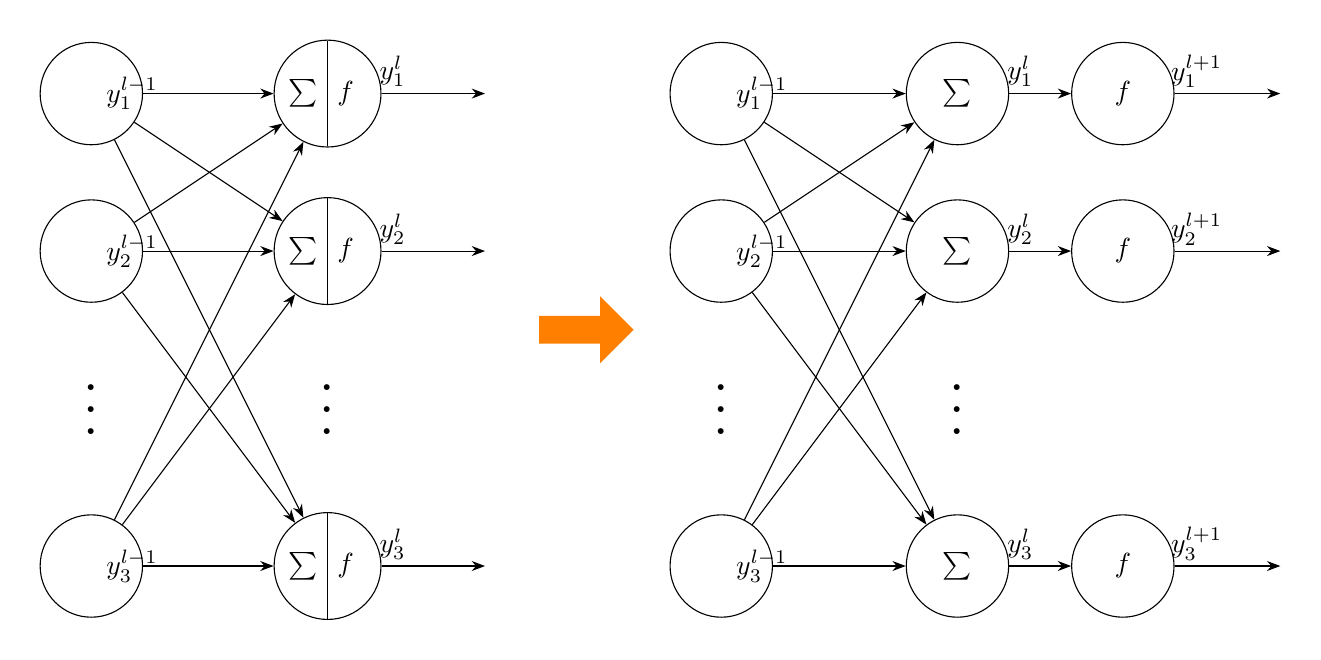
\begin{tikzpicture}[
    background rectangle/.style={fill=white},
    show background rectangle,
    neuron/.style={draw, circle, minimum width=1.3cm},
    >=Stealth, every node/.style={shape border uses incircle}]
    \def\xsep{3cm}
    \def\ysep{2cm}

    \begin{scope}
      \foreach \i in {1,2,4} {
        \node [neuron] (p1\i) at (0, {-(\i - 1) * \ysep}) {};

        \node [neuron, circle split, rotate=90]
          (p2\i) at (\xsep, {-(\i - 1) * \ysep}) 
          {\rotatebox{-90}{$\sum$} \nodepart{lower} \rotatebox{-90}{$f$}};

        \node (p3\i) at (2*\xsep, {-(\i - 1) * \ysep}) {};

      }

      \foreach \i/\ilab in {1/1,2/2,4/3} {
        \node at ($(p1\i.east) + (-4pt, 0)$) {$y_{\ilab}^{l-1}$};
        \node at ($(p2\i.south) + (4pt, 8pt)$) {$y_{\ilab}^{l}$};
        \foreach \j in {1,2,4} {
          \draw[->] (p1\i) -- (p2\j);
        }
        \draw[->] (p2\i) -- ($(p2\i)!2cm!(p3\i)$);
      }

      \foreach \i in {1,2} {
        \node [scale=2, yshift=0.1cm] at ($(p\i2)!0.5!(p\i4)$) {$\vdots$};
      }
    \end{scope}

    \node [fill=orange, single arrow, minimum height=1.2cm] at (6.2cm, -1.5*\ysep) {};

    \begin{scope}[xshift=8cm]
      \foreach \i in {1,2,4} {
        \node [neuron] (p1\i) at (0, {-(\i - 1) * \ysep}) {};
        \node [neuron] (p2\i) at (\xsep, {-(\i - 1) * \ysep})  {$\sum$};
        \node [neuron] (p3\i) at (1.7*\xsep, {-(\i - 1) * \ysep})  {$f$};
        \node (p4\i) at (2*\xsep, {-(\i - 1) * \ysep}) {};
      }

      \foreach \i/\ilab in {1/1,2/2,4/3} {
        \node at ($(p1\i.east) + (-4pt, 0)$) {$y_{\ilab}^{l-1}$};
        \node at ($(p2\i.east) + (4pt, 8pt)$) {$y_{\ilab}^{l}$};
        \node at ($(p3\i.east) + (8pt, 8pt)$) {$y_{\ilab}^{l+1}$};
        \foreach \j in {1,2,4} {
          \draw[->] (p1\i) -- (p2\j);
        }
        \draw[->] (p2\i) -- (p3\i);
        \draw[->] (p3\i) -- ($(p3\i)!2cm!(p4\i)$);
      }

      \foreach \i in {1,2} {
        \node [scale=2, yshift=0.1cm] at ($(p\i2)!0.5!(p\i4)$) {$\vdots$};
      }
    \end{scope}

  \end{tikzpicture}
\end{document}
